\documentclass[aspectratio=169]{beamer}
\setbeamertemplate{navigation symbols}{}
\usepackage{color,amsmath,comment, subfigure}
\usepackage{booktabs}
\def\vf{\vfill}
\usepackage{url}

%\setbeameroption{show notes}

%%%%%%%%%%%%%%%%%%%%%%%%%%
\title[]{Lecture 6: Foci}
\author[]{Matthew Salganik}
\institute[]{Sociology 204: Social Networks, Spring 2021\\Princeton University}
\date[]{
2/3: Social structure

\vfill

\begin{flushleft}
\vspace{0.7in}

\includegraphics[width=0.05\textwidth]{figures/cc.png}
\end{flushleft}
}

\begin{document}
%%%%%%%%%%%%%%%%%%%%%%%%%%%
\frame{\titlepage}
%%%%%%%%%%%%%%%%%%%%%%%%%%%
\begin{comment}
\begin{frame}

SWBAT:
\begin{enumerate}
\item realize the power of edges that don't exist
\item compare psychological vs sociological explanations for network structure
\item apply the idea of foci to understand their personal networks 
\item see how sociological principles can shape the design of technical systems
\end{enumerate}

\end{frame}
\end{comment}
%%%%%%%%%%%%%%%%%%%%%%%%
\begin{frame}

Affiliation network
\begin{figure}
  \centering
  \includegraphics[width=0.75\textwidth]{figures_book/4_6_bi.png}
\end{figure}
\pause
\begin{itemize}
\item actors and movies
\pause
\item scientists and papers
\pause
\item board members and boards of directors
\end{itemize}

\note{
Looking only at the network of relationships, you can get confused.  The real driver is the combination of people and foci.

Feld work helps us think about foci, overlap of foci, and how they create ties.
}

\end{frame}
%%%%%%%%%%%%%%%%%%%%%%%%%%
\begin{frame}

\begin{figure}
  \centering
  \includegraphics[width=0.75\textwidth]{figures_book/4_6_bi_group.png}
\end{figure}

\end{frame}
%%%%%%%%%%%%%%%%%%%%%%%%%%
\begin{frame}

\begin{figure}
  \centering
  \includegraphics[width=0.75\textwidth]{figures_book/4_6_bi_actor.png}
\end{figure}

\end{frame}
%%%%%%%%%%%%%%%%%%%%%%%%%%
\begin{frame}

\begin{figure}
  \centering
  
\includegraphics[width=0.8\textwidth]{figures/feld_focused_1981_title}
\end{figure}

\pause

\begin{itemize}
\item you are stepping in a conversation
\pause
\item a very dense---but interesting---conversation
\end{itemize}

\end{frame}
%%%%%%%%%%%%%%%%%%%%%%%%%%%
\begin{frame}

Foci: a social, psychological, or physical entity around which joint activities are organized. 

\end{frame}
%%%%%%%%%%%%%%%%%%%%%%%%%%%
\begin{frame}

\begin{center}
 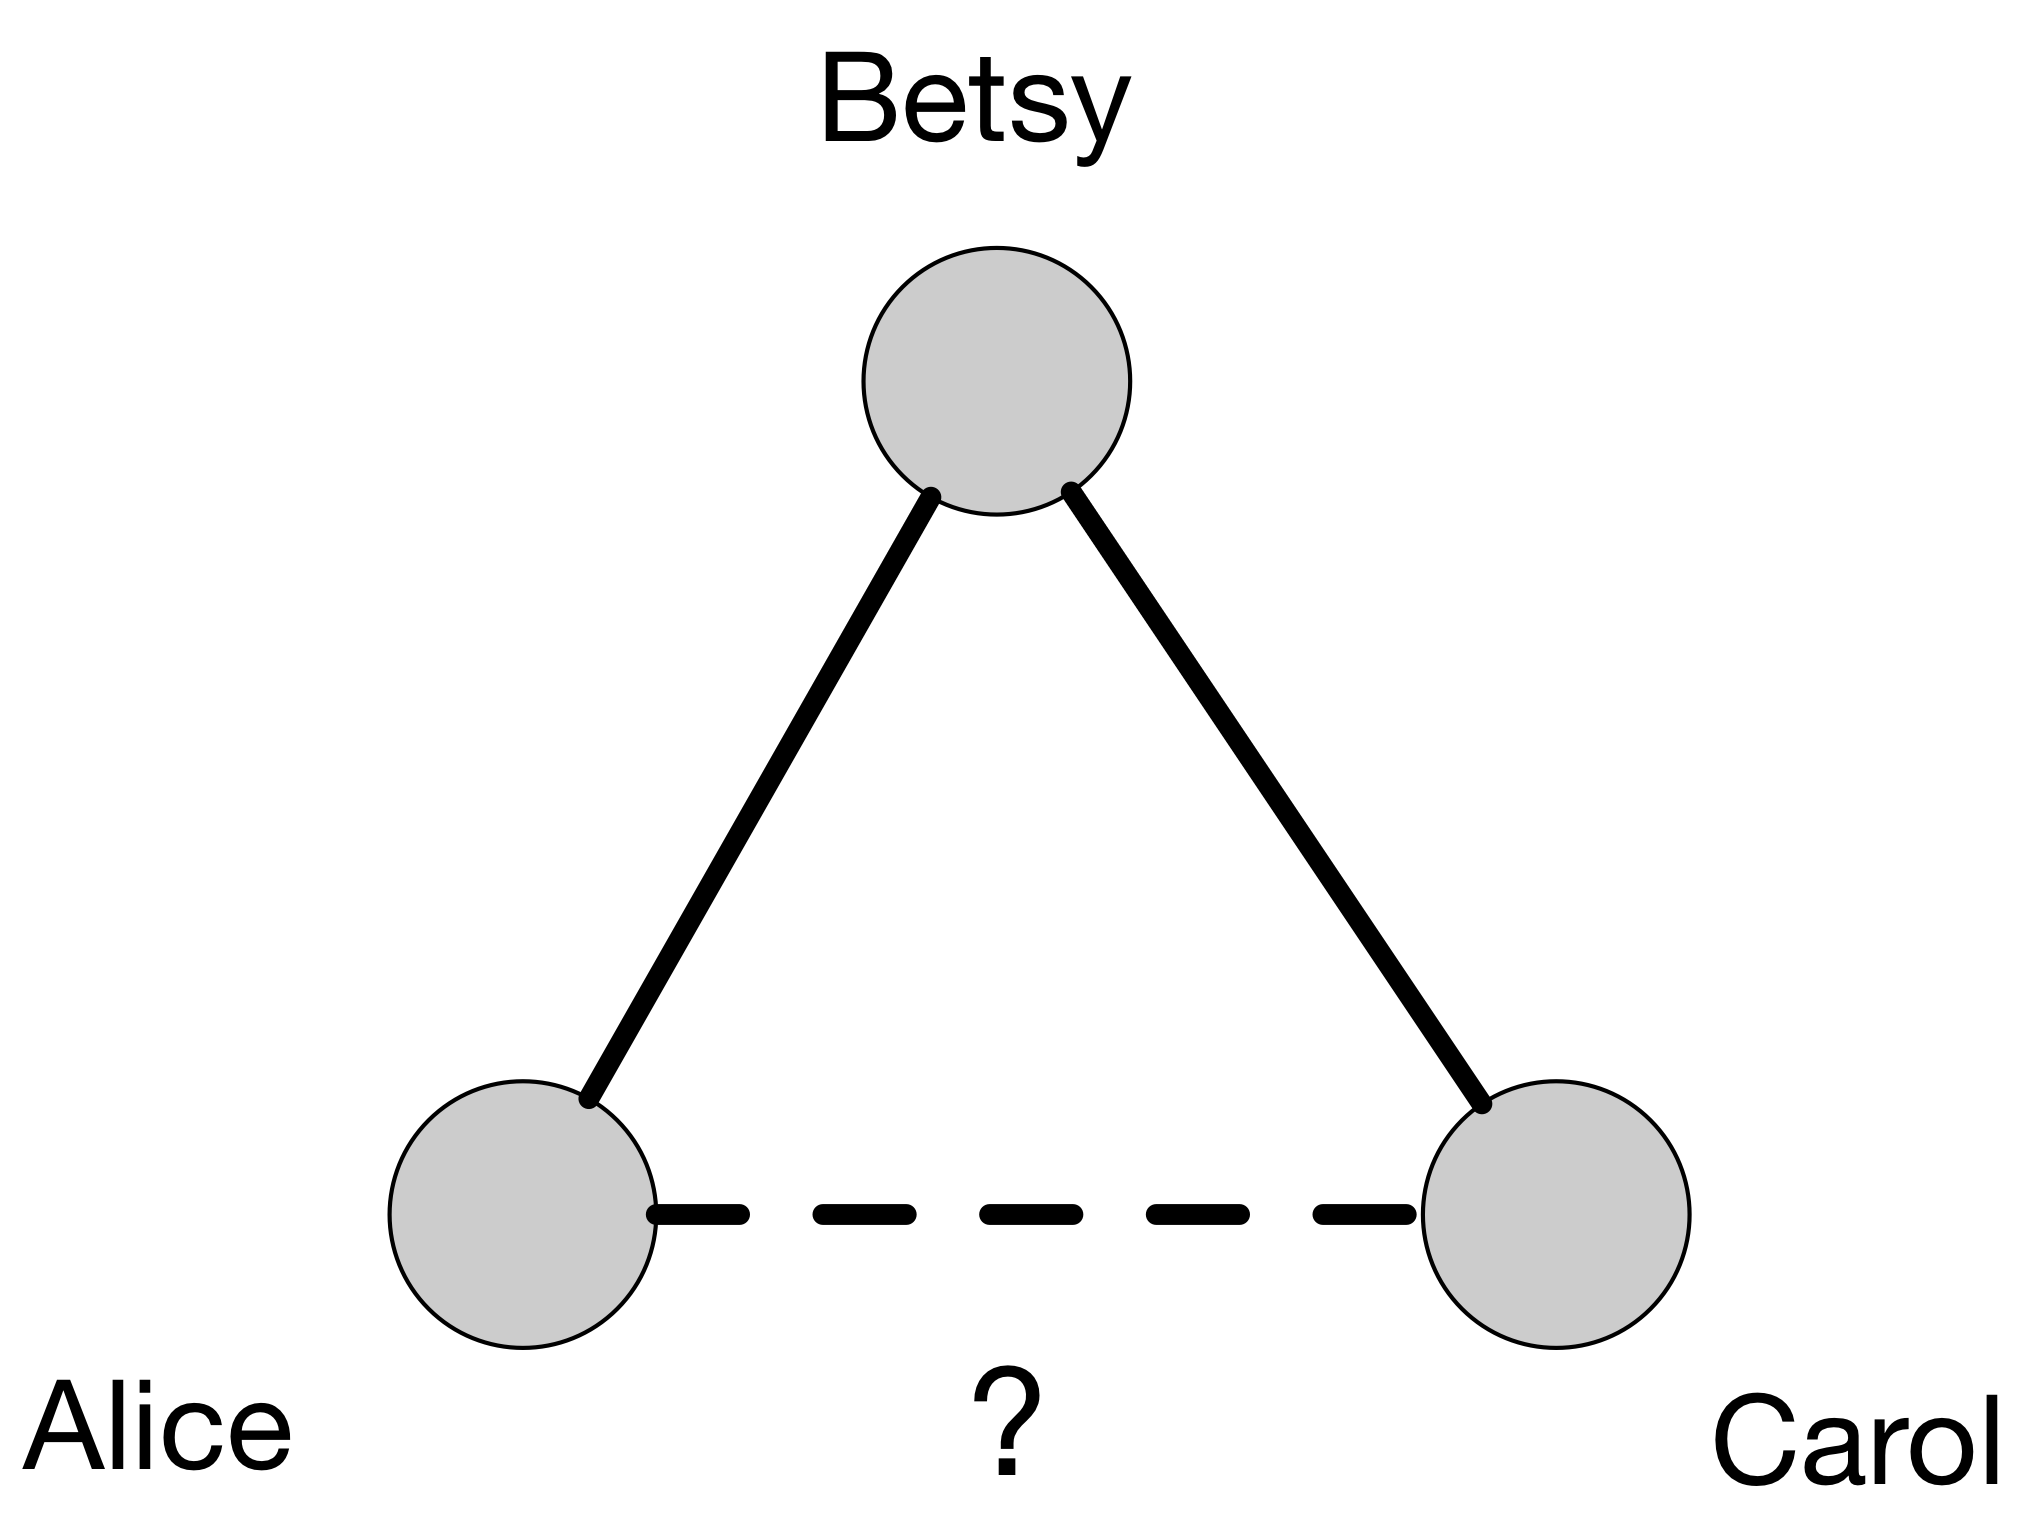
\includegraphics[width=0.6\textwidth]{figures/triadic_closure}
\end{center}

Explaining triadic closure:
\begin{itemize}
\item balance theory vs foci
\item psychology vs sociology
\item agency vs structure
\end{itemize}

\note{
This contrast is clear in Feld when he compares foci to balance theory. 
Balance theory (Heider), psychological process:\\
If Alice likes Betsy and Betsy likes Carol then Alice should like Carol to bring their relationship into to ``balance''\\
Feld said no.  Social structure not psychology\\
This is an example of more broader shift in the way to think about the world sociology over psychology, structure over agency
}

\end{frame}
%%%%%%%%%%%%%%%%%%%%%%%%%%%
\begin{frame}

\begin{center}
{\Large Roughly speaking: you don't pick your friends, your environment picks your friends for you}
\end{center}

\end{frame}
%%%%%%%%%%%%%%%%%%%%%%%%%%%%
\begin{frame}

\begin{center}

\includegraphics[width=0.95\textwidth]{figures/segal_alphabet_1974_title}
\end{center}

\vfill
\url{http://dx.doi.org/10.1037/h0037446}

\end{frame}
%%%%%%%%%%%%%%%%%%%%%%%%%%%%
\begin{frame}

\begin{center}
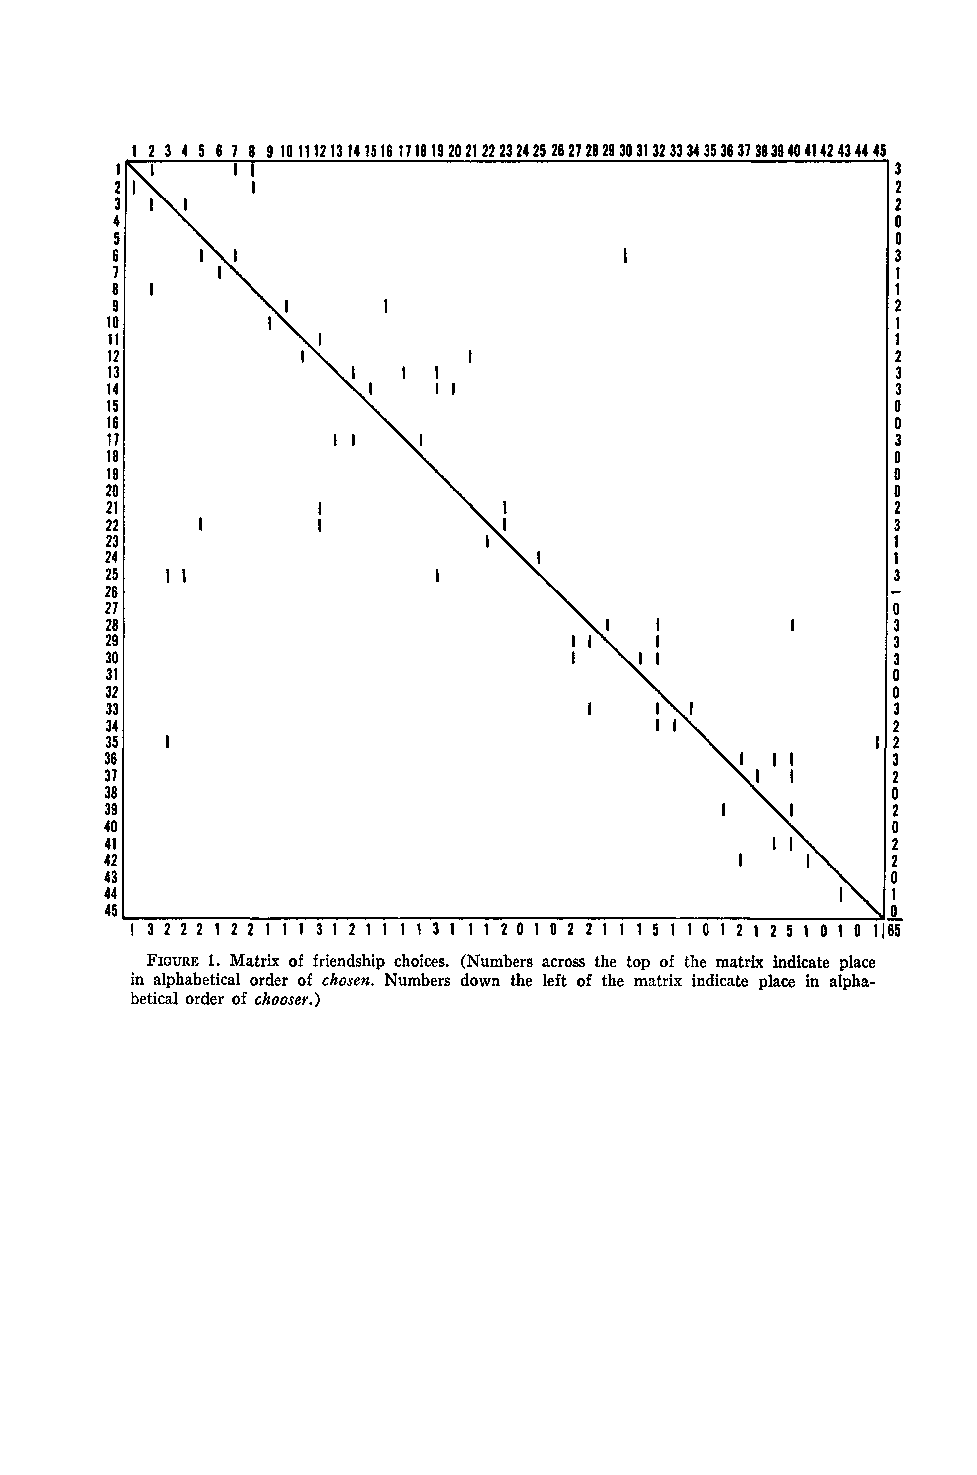
\includegraphics[width=0.6\textwidth]{figures/segal_alphabet_1974_fig1}
\end{center}

\end{frame}
%%%%%%%%%%%%%%%%%%%%%%%%%%%%
\begin{frame}

\begin{center}
 
\includegraphics[width=0.8\textwidth]{figures/bossard_residential_1932_title}
\end{center}

\begin{itemize}
\item study of 5,000 marriage licenses in which one or both applicant lived in Philadelphia (January - May 1931)
\end{itemize}

\vfill
\url{https://www.jstor.org/stable/2766455 }

\end{frame}
%%%%%%%%%%%%%%%%%%%%%%%%%%%
\begin{frame}

\begin{center}
 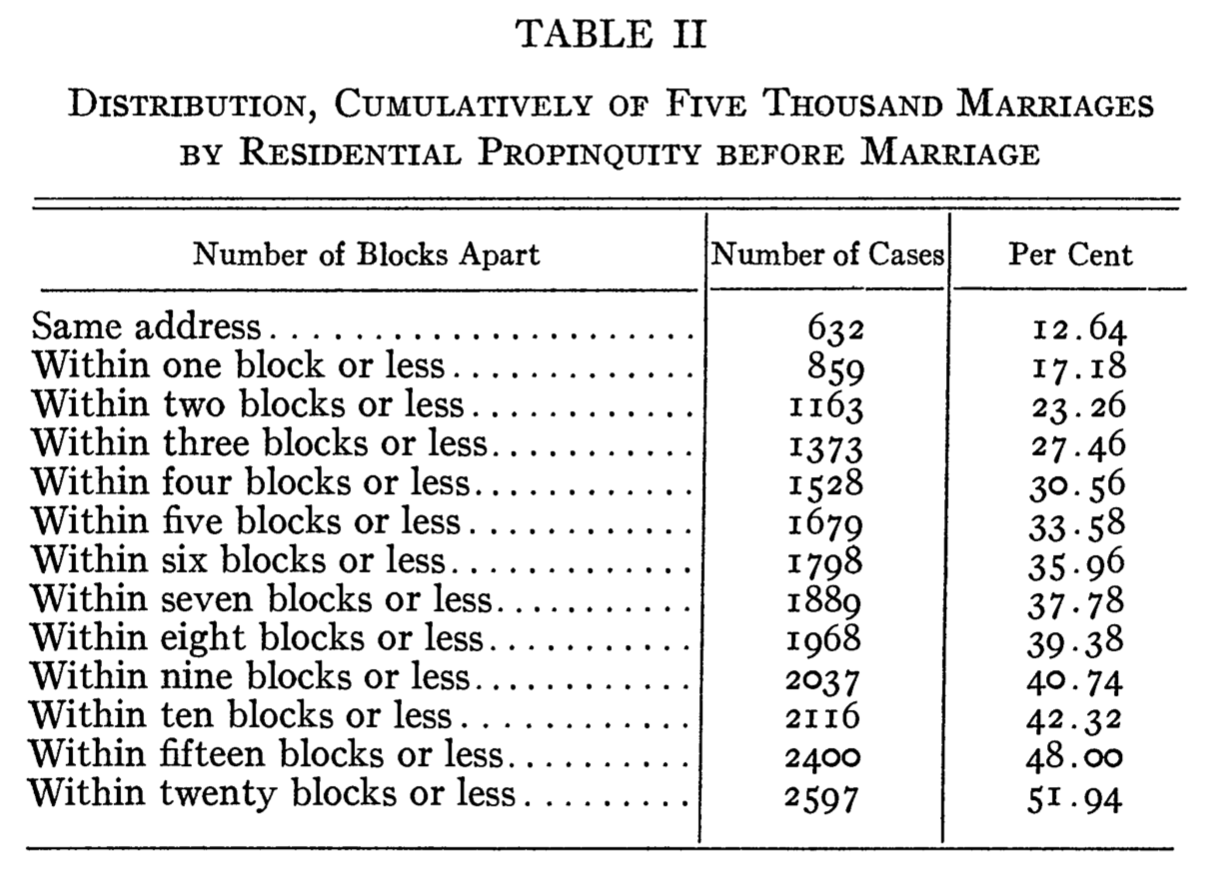
\includegraphics[height=0.7\textheight]{figures/bossard_residential_1932_tab2}
\end{center}

\begin{itemize}
\item More than one in three couples involved a person lived within 5 blocks or less. 
\pause
\item Bossard (1932): ``Cupid may have wings, but apparently they are not adapted for long flights.''
\end{itemize}

\note{
Things not as extreme as in 1932 but geography still plays a huge role in the formational of relationships
}

\end{frame}
%%%%%%%%%%%%%%%%%%%%%%%%%%%
\begin{frame}

\begin{itemize}
\item The theory of foci calls attention to the fact that many network ties are formed because of social structure.
\pause
\item What do foci have to do with Facebook and Google+?
\end{itemize}

\end{frame}

\end{document}
